\documentclass[11pt, a4paper]{article}
\input{preamble.tex}
\switchlang{en}
\begin{document}

\title{1984 -- Dave Brown Dual Joystick}
\date{}
\author{~}
\maketitle
\selectlanguage{english}

The Dave Brown Dual Joystick (fig. \ref{fig:DaveBrownJoystickPic}) is actually a  two-axis joystick that copies the appearance and design features of radio-controlled model airplane controllers from the 1980s. However, instead of being used with radio control, the joystick is a wired one, designed specifically for Dave Brown RC Flight Simulator, a flight simulator program written by model aircraft enthusiast John Kalend \cite{Kallend1, Kallend2}. This flight simulator was available on Apple II and Commodore 64 computers in the first half of 1980s, and even longer on IBM-compatible computers (boxed versions of Dave Brown R/C Simulator from 1995 are available with the same joystick model inside). Within the simulation, the joystick allows control of flight parameters, including roll, pitch, speed, and altitude, similar to how this is implemented in radio-controlled models. According to the documentation, the joystick had its own name, ``Transmitter'' \cite{Joystick1}.

\begin{figure}[h]
   \centering
    
\includegraphics[width=\textwidth]{1984_dave_brown_dual_joystick/pic_30.jpg}
    \caption{Dave Brown Dual joystick}
    \label{fig:DaveBrownJoystickPic}
\end{figure}

As mentioned, the device's body mimics the appearance and layout of aircraft R/C models remote control: it is a large metal  rectangular block with two independent sticks, as seen in fig. \ref{fig:DaveBrownJoystickTopAndBottom}. The underside of the body is completely flat, without any elements, including feet. On the top side, there are two independent sticks (each with its own pair of trimmers for mechanically adjusting the central position along both axes), and two red toggle buttons with locking latches. Another button is located on the side of the body (the one far from the user). The joystick is connected to a computer with two cables: one cable corresponds to the left joystick, the other to the right.

\begin{figure}[h]
    \centering
    
\includegraphics[scale=0.47]{1984_dave_brown_dual_joystick/top_15.jpg}
    
\includegraphics[scale=0.47]{1984_dave_brown_dual_joystick/bottom_15.jpg}
    \caption{Dave Brown Dual joystick, top and bottom views}
    \label{fig:DaveBrownJoystickTopAndBottom}
\end{figure}

The body size and ergonomics can be assessed by looking at the figures \ref{fig:DaveBrownJoystickSize} and \ref{fig:DaveBrownJoystickHand}.

The stick and the whole mechanical unit is a standard component: it can be found on some compact analog joysticks from other companies of the time, including the very first Joystick for Apple II, developed by Jef Raskin and later available under the A2D Company brand. Sticks are quite comfortable to move when gripped with your fingers, while the palm rests on the body (fig. \ref{fig:DaveBrownJoystickHand}), which is not the case with the miniature buttons.

\begin{figure}[h]
    \centering
    
\includegraphics[scale=0.49]{1984_dave_brown_dual_joystick/size_15.jpg}
    \caption{Dave Brown Dual joystick on a graduated pad with a grid step of 1~cm}
    \label{fig:DaveBrownJoystickSize}
\end{figure}

Fortunately for the user, the buttons usage is not as intensive as in most computer games. Within the simulation, the user is given control over flight parameters, including roll, pitch, airspeed, and altitude. According to the documentation, the game reproduces the fundamental physics of model aircraft flight and allows for basic maneuvers such as loops and rolls, helping to develop rudder memory for controlling real models \cite{Joystick2}. The device replicates the control mode most common in radio-controlled model airplanes of its time \cite{Joystick1}. Throttle is controlled by moving the left stick forward and backward, rudder (yaw) is controlled by moving the left stick left and right, elevator (pitch) is controlled by moving the right stick forward and backward (pulling it back to raise the elevator), and aileron (roll) is controlled by moving the right stick left and right. The left button, when in pressed state, halves the sensitivity of the elevator axis, while the right button has the same effect on aileron control. The instructions do not disclose the purpose of the third button.

\begin{figure}[h]
    \centering
    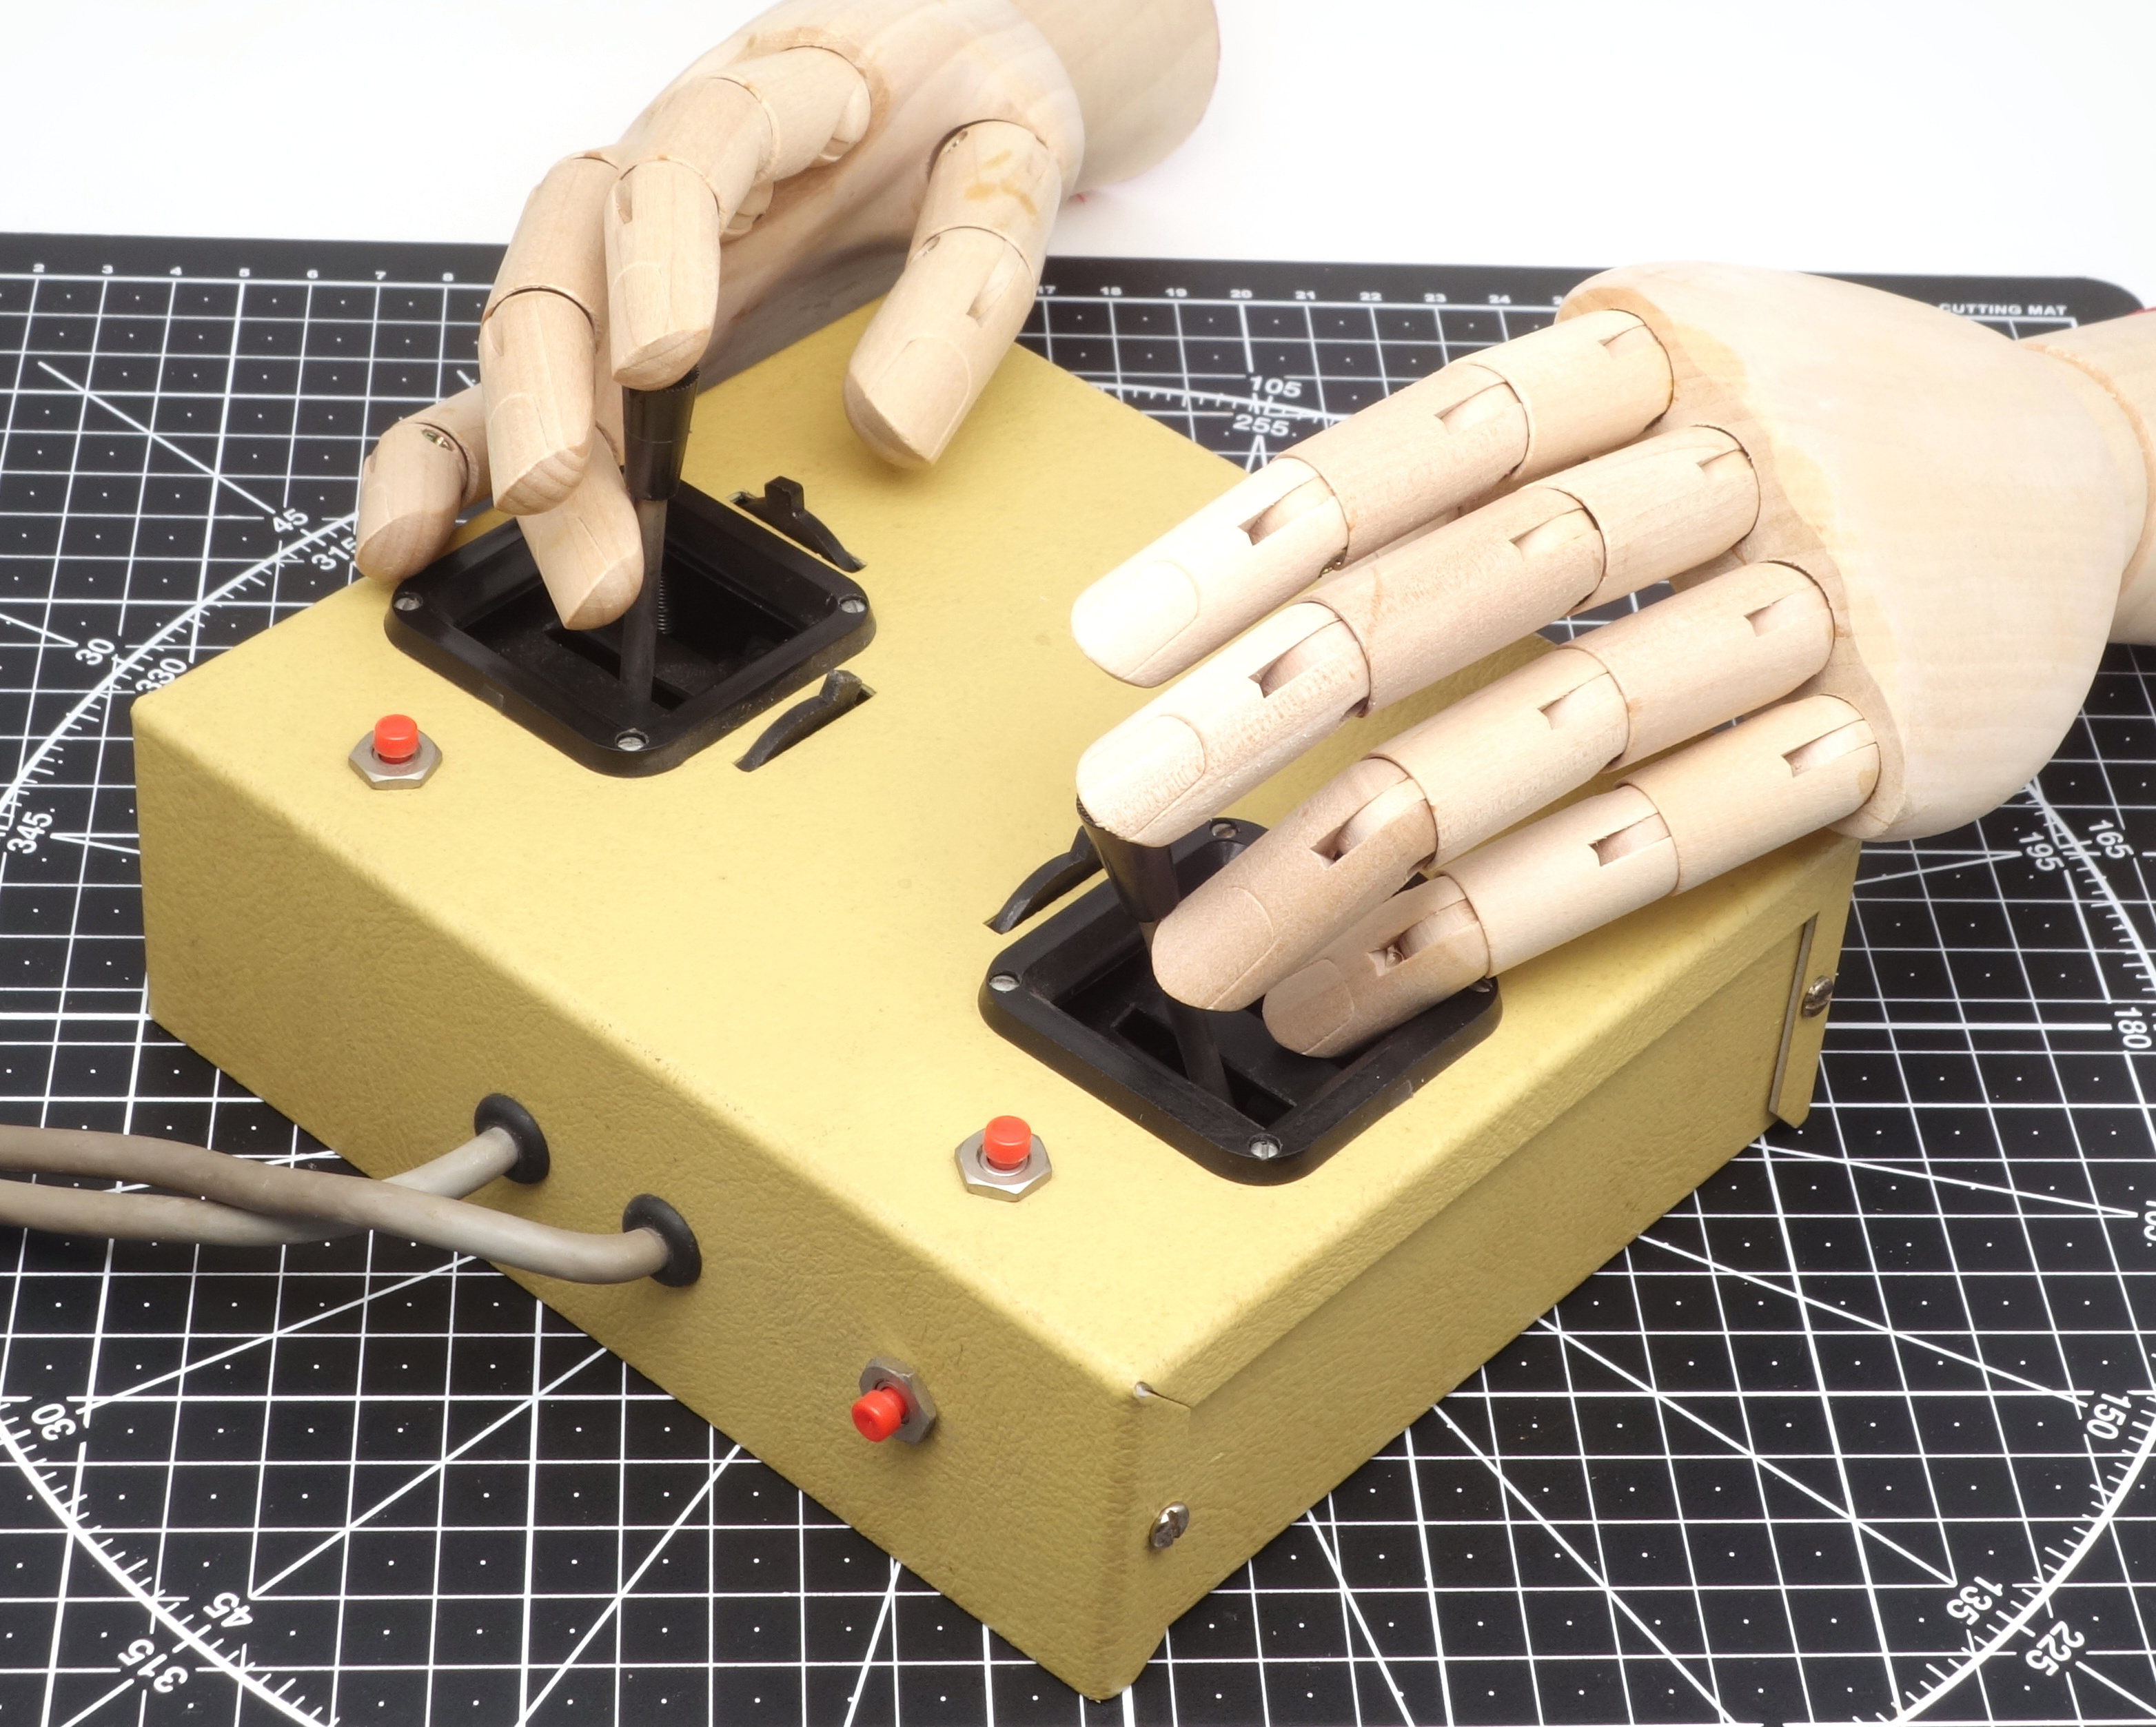
\includegraphics[scale=0.49]{1984_dave_brown_dual_joystick/hand_15.jpg}
    \caption{Dave Brown Dual joystick with a human hand model}
    \label{fig:DaveBrownJoystickHand}
\end{figure}

R/C Flight Simulator is designed to simulate the control of radio-controlled aircraft on the screens of 8-bit home computers such as the Apple II and Commodore 64 \cite{Joystick2}.

As the \cite{Joystick1} manual explains, ``the user is presented with a realistic, animated image of the model as it `flies', as if taken by a TV camera located on the ground at the pilot's feet''. The same manual goes on to explain that ``this program is very complex, solving the differential equations of flight, and then generating the 3-D graphics in real time'', but ``some simplification had to be made, in order to enable the program to runat reasonable speed on a microcomputer''. Naturally, the computing capabilities of 8-bit home computers brought their limitations: a first impression of its graphical features and level of detail can be obtained from a screenshot shown in the figure \ref{fig:game}, and a more complete overview can be found, for example, in the online version of the game \cite{simulator}. The software is also interesting because its author, John Kallend, is likely one of the oldest R/C model enthusiasts. In any case, the blog he maintained at \url{https://rcgroups.com} after retiring as a professor of the  Metalurgical and Materials Engineering Department at the Illinois Institute of Technology was active until June 2025, and the author's comment under A nickname modestly stated ``Flying R/C since 1964'' \cite{Kallend1}.

\begin{figure}[h]
    \centering
    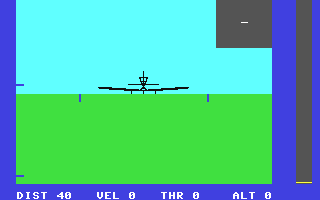
\includegraphics[scale=1]{1984_dave_brown_dual_joystick/screen.png}
    \caption{R/C Flight Simulator screenshot} \label{fig:game}
\end{figure}

The internal design of the Dave Brown Dual Joystick is shown in fig. \ref{fig:DaveBrownJoystickInside}. The joysticks are mounted on metal gimbals, providing smooth control along two axes. Each joystick is connected to a potentiometer, converting the deflection of the stick into a change in resistance. The analog port of the Apple II and Commodore 64 \cite{Joystick1} measured the charge time of the RC circuit, allowing the software to determine the absolute position of the joystick.

\begin{figure}[h]
    \centering
    
\includegraphics[width=\textwidth]{1984_dave_brown_dual_joystick/inside_30.jpg}
    \caption{Dave Brown Dual joystick disassembled}
    \label{fig:DaveBrownJoystickInside}
\end{figure}

\begin{thebibliography}{9}
\bibitem {Joystick1} Radio Controlled Flight Simulator By John Kallend For Commodore 64. \url{https://raw.githubusercontent.com/fiowro/mouses/main/source/OCR/dave_brown_simulator_joystick.pdf}

\bibitem {Kallend1} kallend's blog. Do It Yourself Afterburner and other stuff -- RC Groups \url{https://www.rcgroups.com/forums/member.php?u=42040}

\bibitem {Kallend2} Kallend J. The Whistler. Builds great... flights quckly... and is different \url{https://www.rcgroups.com/forums/showatt.php?attachmentid=8106951}

\bibitem {Joystick2} Painful Fun Vintage 1980's Dave Brown RC Flight Simulator | HobbyView \url{https://www.youtube.com/watch?v=zqE4cHVLAhk}

\bibitem {simulator} Pay RFC64 -- Radio controlled flight sumulator. CommodoreGames.Net \url{https://www.commodoregames.net/Commodore64/RCFS-64-Radio-Controlled-Flight-Simulator-28134.html}
\end{thebibliography}
\end{document}
